%\documentclass[a4paper,10pt]{report}
\documentclass[11pt,titelpage]{scrartcl}
\usepackage[utf8]{inputenc}
\usepackage[ngerman]{babel}
\usepackage{graphicx}
\usepackage{fancyhdr}
\usepackage{fancyref}
\usepackage{hyperref}
\usepackage{lscape}
\usepackage{color}
\usepackage{pgfgantt}
\usepackage{lscape}
\definecolor{javared}{rgb}{0.6,0,0} % for strings
\definecolor{javagreen}{rgb}{0.25,0.5,0.35} % comments
\definecolor{javapurple}{rgb}{0.5,0,0.35} % keywords
\definecolor{javadocblue}{rgb}{0.25,0.35,0.75} % javadoc
\definecolor{javared}{rgb}{0.6,0,0} % for strings
\definecolor{lightgrey}{rgb}{0.97,0.97,0.97}
\definecolor{grey}{rgb}{0.3,0.3,0.3}
\definecolor{darkgreen}{rgb}{0,0.6,0}

\usepackage{listings}
\lstset{
language=java,
keywordstyle=\color{javapurple}\bfseries,
stringstyle=\color{javared},
commentstyle=\color{javagreen},
morecomment=[s][\color{javadocblue}]{/**}{*/},
numberstyle=\tiny\color{grey},
numberfirstline=true,
firstnumber=1,
stepnumber=5,
numbers=left,
numbersep=10pt,
tabsize=4,
breaklines=true,
showspaces=false,
showstringspaces=false,
backgroundcolor=\color{lightgrey}
}


%must be before gloassary stuff\usepackage{hyperref}
\usepackage[toc]{glossaries}

%\makeglossaries
%
\newglossaryentry{Buildystem}
{
  name=Buildystem,
  description={Linux Mint 17, Java JDK 1.8.1, Intellij 2016.3.5, JavaFx Scene Builder 2.0}
} 

\newglossaryentry{Referenzsystem}
{
  name=Referenzsystem,
  description={Linux Mint 17, Java JRE 1.8.1, Derby10.13.1.1}
} 

\newglossaryentry{Programmstart}
{
  name=Programmstart,
  description={Prozess welcher das Programm initialisiert}
} 


 
\newglossaryentry{Standarddatenbank}
{
  name=Standarddatenbank,
  description={Derby, MySQL, SQLite}
} 


\newglossaryentry{JPA Driver}
{
  name=JPA Driver,
  description={JPA Driver und JPA Module sind Opensource CMS (Content Management Systeme)}
} 

\newglossaryentry{Benutzer}
{
  name=Benutzer,
  description={Ein Benutzer ist ein Mensch, welcher unser Programm benutzt. Falls nicht anders erwähnt, muss dieser
  weder registriert noch angemeldet sein}
} 


\newglossaryentry{Event}
{
  name=Event,
  description={Ein Event ist ein Ereignis, welches zu einem bestimmten Zeitpunkt stattfindet}
} 

\newglossaryentry{Einzelevent}
{
  name=Einzelevent,
  description={Ein Einzelevent ist ein Event, welches nicht periodisch wiederkehrend stattfindet, also können auch
   ein Treffen, welches unregelmässig stattfindet zu einem Einzelevent werden.}
} 

\newglossaryentry{GUI}
{
  name=GUI,
  description={Graphical User Interface. Ein GUI ist eine Graphische Benutzeroberfläche. Sie hat die Aufgabe das
  Programm für den Benutzer bedienbar zu machen}
} 

\newglossaryentry{CLI Wikipedia}
{
  name=CLI,
  description={Command Line Interface. Das CLI ist die Konsole, wird oft auch Terminal gennant. Sie steuert eine
  Software mittels Textmodus. Je nach Betriebssystem wird die Kommandozeile von einer Shell ausgewertet und die
  entsprechende Funktion ausgeführt.
  - Wikipedia}
}

\newglossaryentry{Shell}
{
  name=Shell,
  description={In der Informatik bezeichnet man als Shell die Software, die den Benutzer mit dem Computer verbindet.
  Die Shell ermöglicht zum Beispiel, Kerneldienste zu nutzen und sich über Systemkomponenten zu informieren oder sie zu
  bedienen. Die Shell ist in der Regel ein Teil des Betriebssystems.
  - Wikipedia
  }
}


\newglossaryentry{API}
{
  name=API,
  description={Application Programming Interface. Ein API ist ein Programmteil, der von einem Softwaresystem anderen
  Programmen zur Anbindung an das System zur Verfügung gestellt wird
  - Wikipedia}
} 

\newglossaryentry{Notification}
{
  name=Notification,
  description={Eine Notification ist eine Aktion des Programms, die den Benutzer auf ein Event aufmerksam machen soll.}
} 

\newglossaryentry{Konfiguration}
{
  name=Konfiguration,
  description={Die Konfiguration kann ein Programm auf die Bedürfnisse des Nutzers anpassen. So kann man beispielsweise
   die Spracheinstellung konfigurieren.}
} 

\newglossaryentry{Filtern}
{
  name=Filtern,
  description={Filtern bedeutet, dass man gewisse Informationen nur darstellt, wenn diese eine oder mehrere bestimmte Charakteristiken aufweist. So ist es zum Beispiel möglich Events nach Kategorein zu filtern, so dass man nur Events aus einer bestimmten Kategorie sehen kann.}
} 


\newglossaryentry{Kategorien}
{
  name=Kategorien,
  description={Eine Kategorie hilft die Events zu klassieren. Denkbare Kategoreien sind zum Beispiel: Arbeit, Freizeit, Persönlich,Familie,Wichtig,Sportverein... }
} 

\newglossaryentry{Android}
{
  name=Android,
  description={Android ist ein Betriebssystem für Mobile Geräte wie Smartphones, Tablets etc.
   Es wird von der von Google gegründeten Open Handset Alliance entwickelt}
}

\newglossaryentry{Notification Infrastruktur}
{
  name=Notification Infrastruktur,
  description={Einige Desktop Environments  wie Gnome oder KDE bieten eine eigene Notification Infrastruktur, diese erlaubt es ``Pop-Ups'' durch Systemkomponenten darzustellen. KDE benutzt dies beispielsweise um auf einen Niedrigen Batterieladezustand hinzuweisen. Auch andere Programme können diese Notification Infrastruktur nutzen. }
} 

\newglossaryentry{Desktop Environment}
{
  name=Desktop Environment,
  description={Deskto Environment, ist eine Graphsche Benutzeroberfläche für das Betriebssystem. Vorallem unter
  Unixoiden Betriebssystemen, hat man eine grosse Auswahl an Desktop Environments (KDE, gnome, w3..)}
} 

\newglossaryentry{Cronjob}
{
  name=Cronjob,
  description={Cronjob ist ein Unix Dienst, welcher dazu dient zu einem bestimmten Zeitpnkt Ereignisse auszulösen.}
} 



\newglossaryentry{IFTTT}
{
  name=IFTTT,
  description={IFTTT (die Abkürzung von If This Then That, ausgesprochen „ift“ wie in „Gift“[1]) ist ein Dienstanbieter,
  der es Benutzern erlaubt, verschiedene Webanwendungen (zum Beispiel Facebook, Evernote, Dropbox usw.) mit einfachen
  bedingten Anweisungen zu verknüpfen.
   -Wikipedia}
} 








% Title Page
\title{Alarm Clock: Arbeitsprozess }
\author{Jonathan Hyams \\Pascal Schmalz}
\titlehead{\centering
\includegraphics[width=6cm]{../Requirements/img/clock.png}}
%\titlehead{\centering
\includegraphics[width=6cm]{img/clock.png}}

%Make the Header
\makeatletter
\let\runauthor\@author
\let\runtitle\@title
\makeatother
\rhead{\runauthor}
\chead{\runtitle}
%\lhead{\begin{picture}(0,0) \put(0,0){
\includegraphics[scale=0.5]{img/bfh.png}} \end{picture}}


\begin{document}

\thispagestyle{empty}
\maketitle
\pagebreak
\tableofcontents

\pagestyle{fancy}


\begin{abstract}
\end{abstract}
\pagebreak


\section{Zweck des Dokument}
Dieses Dokument dient dem Leser zur Klarstellung, wie wir das Projekt angegangen sind, wie wir es geplant haben und wo wir Schwierigkeiten hatten.
\subsection{Planung}
Als erstes sind wir Zusammengesessen und haben uns Überlegt, was unser Projekt braucht, um ein anständigen AlarmClock zu werden. Dafür sind wir
vor einer Wandtafel gestanden und haben Stichworte aufgeschriebe die wir dann in den Code einbauen wollen. Darunter waren Stichwörter wie
Email, Datenbanken, Shellscripts und Cronjobs eingeflossen. Daraus haben wir dann ein UML designed das aufzeigt , wie wir das Ganze aufbauen wollen (Abbildung 1).
\begin{landscape}
\begin{figure}
  \centering
    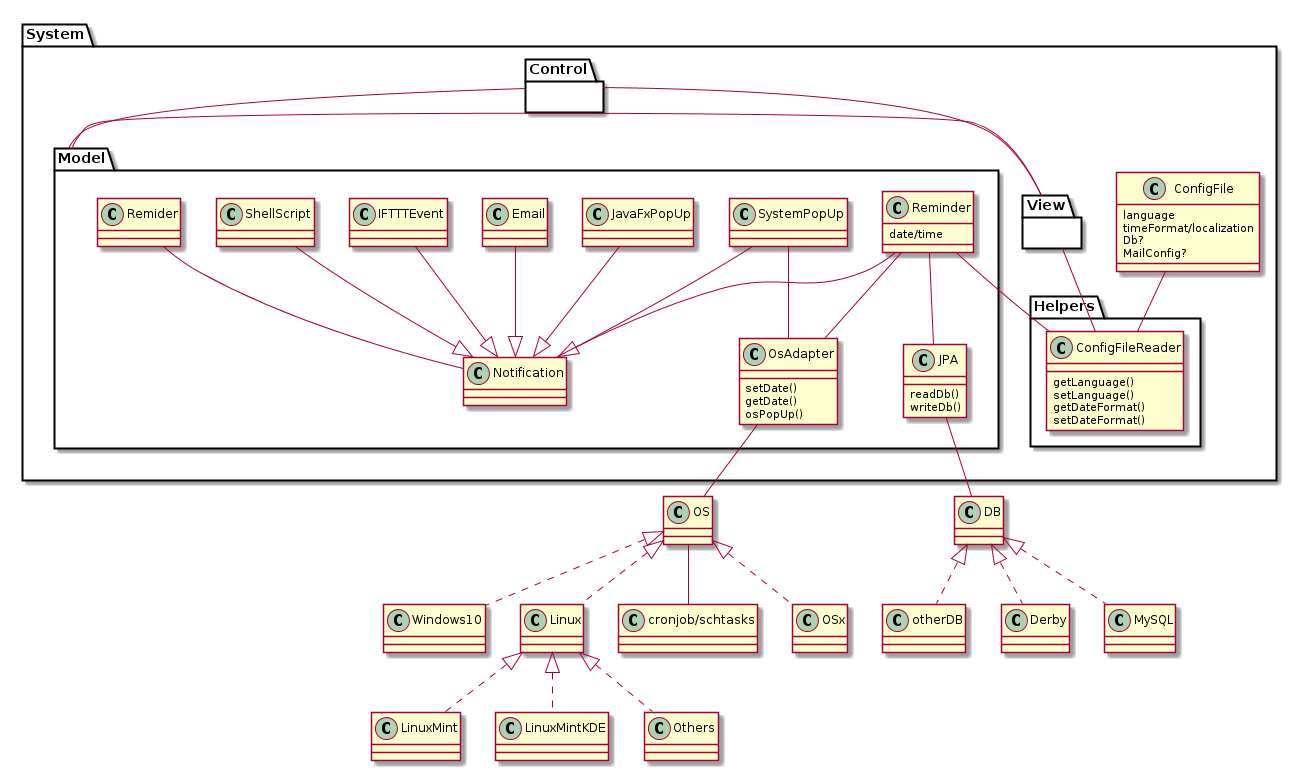
\includegraphics[width=1\textwidth]{../uml/uebersicht00.png}
  \caption{Systemübersicht Version 1}
  \label{fig:overview}
\end{figure}
\end{landscape}
Dieses UML-Diagramm haben wir dann auch Herr Prof. Fuhrer gezeigt, welcher es zwar eine Gute Idee fand, aber sagte dass wir das nie in der gegebenenen
Zeit schaffen werden. Sachen wie Cronjobs, Shellscripts und verschiede Datenbanken daranzunängen wäre für uns unmöglich.
Also haben wir nochmal von Vorne angefangen und sind mit einem überarbeitetem UML vorangegangen (Abbildung 2).

\begin{figure}
  \centering
    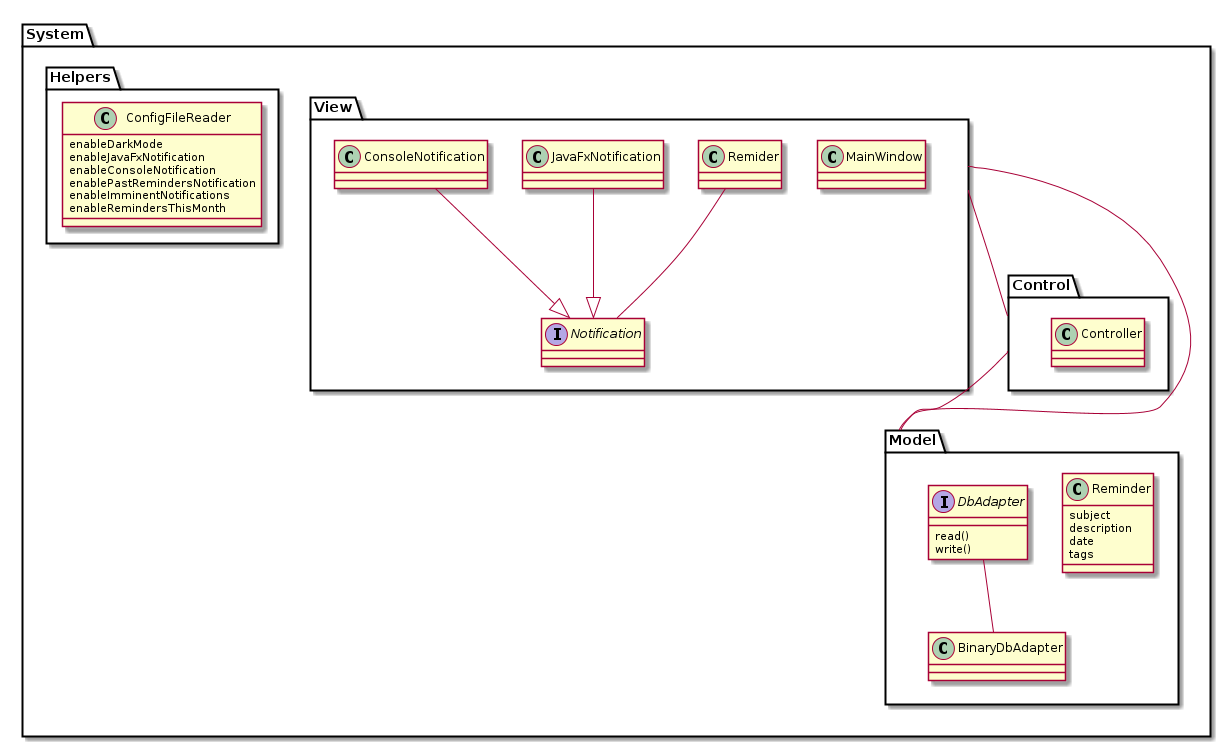
\includegraphics[width=1\textwidth]{../uml/uebersicht01.png}
  \caption{Systemübersicht Version 2}
  \label{fig:overview}
\end{figure}
Danach haben wir uns überlegt, was für Meilenstein wir uns setzen wollen:
\begin{enumerate}
  \item Ein GUI mit einer Tabelle von Reminders
  \item Abspeichern der Daten mittels einer Datenbank (wir haben uns für ein binäres Serialisieren entschieden)
  \item Ein Poller der immer wieder überprüft ob ein Reminder eingetroffen ist
  \item Notifications die den User über die Konsole zeigen das ein Reminder eingetroffen ist
  \item JavaFX Popups die dem User zeigen das ein Reminder eingetroffen ist
\end{enumerate}
Anschliessend haben wir begonnen uns hinter das Codieren zu Setzen. 2 Wochen vor der Abgabe des Codes, haben mit der Dokumentation des Codes angefangen.
\subsection{Deliverables}
Von uns wurde verlangt, dass wir einen Betriebssystemunabhängigen Open Source Alarm Clock bauen, der wie kAlarm aufgebaut ist.
Es sollte
\begin{itemize}
  \item Widerkehrende Events haben
  \item Persistenz
  \item Externes konfigurations File
  \item Datenbank unabhängig
  \item Betriebssystem unabhängig
\end{itemize}
Wiederkehrende Events und Externes Konfigurations File haben wir leider nicht mehr geschafft. Jedoch eine interne Konfigurations Klasse haben wir gebaut.
\begin{landscape}

\subsection{Gantt-Chart}
\label{sub:gantt_chart}


\begin{center}

\begin{ganttchart}[
  vgrid,
  hgrid,
  bar/.append style = {fill = blue!50},
  bar label node/.append style = {left = 5mm},
  milestone label text = \textbf{#1 },
  milestone label node/.append style = {left = 5mm}
  ]{1}{34}
%labels
\gantttitle{\textbf{Projekt 1}}{34} \\
\gantttitle{Kalenderwoche}{34} \\

\gantttitlelist{8,9,10,11,12,13,14,15,16,17,18,19,20,21,22,23,24}{2} \\

\ganttmilestone{Projektstart}{0} \ganttnewline
\ganttbar{Planung}{1}{1} \ganttnewline
\ganttbar{Einlesen}{2}{3} \ganttnewline
\ganttmilestone{Einarbeitung abgeschlossen}{3} \ganttnewline
\ganttbar{GUI Programmieren}{4}{10} \ganttnewline
\ganttbar{Serialisieren}{11}{14} \ganttnewline
\ganttbar{Poller}{15}{16} \ganttnewline
\ganttbar{Notifications}{17}{22} \ganttnewline
\ganttbar{Popups}{23}{28} \ganttnewline
\ganttmilestone{Programmierung abgeschlossen}{28} \ganttnewline
\ganttbar{Präsentation vorbereitung}{29}{30} \ganttnewline
\ganttbar{Dokumentation}{31}{34} \ganttnewline
\ganttmilestone{Projektabschluss}{34}


\ganttlink{elem0}{elem1}
\ganttlink{elem1}{elem2}
\ganttlink{elem2}{elem3}
\ganttlink{elem1}{elem4}
\ganttlink{elem2}{elem4}
\ganttlink{elem3}{elem4}
\ganttlink{elem4}{elem5}
\ganttlink{elem5}{elem6}
\ganttlink{elem6}{elem7}
\ganttlink{elem7}{elem8}
\ganttlink{elem8}{elem9}
\ganttlink{elem9}{elem10}
\ganttlink{elem10}{elem11}
\ganttlink{elem11}{elem12}

\end{ganttchart}
\end{center}
\end{landscape}
Wir haben uns nicht im Voraus überlegt was wie lange dauern wird. Wir haben uns einfach aufgelisten was im Code alles drin sein muss.
\section{Meilensteine}
\subsection{GUI}
Zuerst wollten wir ein brauchbares GUI als Interface haben, da es oftmals einfacher ist Ideen zu diskutieren, wenn man eine Bildilche Diskusionsgrundlage h at. Unser Ziel war es das GUI als optischen Prototypen zu benutzen zu können.

\subsection{Serialisieren}
Der nächste Meilenstein war die Serialisierbarkeit. Wir wollten, dass wir die Reminders speichern könen. Damit kann man sie später wieder von der Festplatte laden.
\subsection{Poller}
Mit dem Poller wollten wir sicherstellen, dass die Notifications auch abgesendet werden, wenn das Programm ``geschlossen'' wurde.
\subsection{Notifications}
Mit den Notifications wollten wir sehen, ob es Funktioniert nach einer vom User bestimmten Zeit eine Notification auf der Konsole zu erhalten.
\subsection{Popups}
Danach wollten wir, wenn die Notification eintrifft, ein JavaFX Popupt erhalten.
\section{Stolpersteine}
\subsection{Gitignore}
\LaTeX generiert beim compilieren recht viele Dateien neben dem gewollten PDF. Diese Dateien wollten wir nicht über git synchronisieren. Es wäre sonnst möglich,dass die Dateien nicht zusammenpassen und beim erneuten compilieren zu einem Fehler führen. Wir wollten die Dateein also ins gitignore file reinnehmen, in welchem man definieren kann, welche Dateien nicht mit git verwlatet werden.
Der gitignore syntax ist aber etwas speziell man kann nicht einfach ein  Verzeichnis ignorieren und dann mittels einer whitelist bestimmte Dateien wieder in die Versionierung mit einbeziehen. Will man ein solches Vehalten erreichen, darf man lediglich den Inhalt der Verzeichnsse ausklammern, und dann mittels Whitelisting wieder in die Versionskontrolle mit einbeziehen. Diesen Sachverhalt genau zu eruieren hat viel Zeit Verschlungen. Als er einmal erkannt wurde, mussten wir trotzdem noch genau darauf achten, dass wir nur genau die Dateien synchronisieren, wleche wir auch synchronisieren wollten.
\subsection{JavaFX serialisieren}
JavaFX Komponenten lassen sich nicht Serialisieren. Bis wir das herausgefunden haben, hat auch einige Stunden gedauert. Um dieses Problem zu umgehen haben wir herausgefunden, dass
wenn man JavaFX Komponenten nicht direkt in der Klasse abspeichert, sonder sie nur zurückgibt, dann funktioniert es. Ein kurzes Beispiel:
Die Table im GUI verlangt nicht Strings, sondern SimpleStringProperties. Das Problem ist aber, dass diese SimpleStringProperties nicht serialisierbar sind.

Falsch:
\begin{lstlisting}
private SimpleStringProperty subject = new SimpleStringProperty();

public SimpleStringProperty getSubjectProperty() {
  return subject;
}
\end{lstlisting}

Richtig:
\begin{lstlisting}
private String subject = "";

public SimpleStringProperty getSubjectProperty() {
  return new SimpleStringProperty(subject);
}
\end{lstlisting}

\subsection{PLatform.runlater}
Ein weiteres Problem das wir hatten war das verspätete Erscheinen von Popups. Wenn man ein Popup z.B. eine Minute nach Programmstart aufruft, hat man effektiv mehrere Dutzend Exceptions bekommen.
Der Grund war, dass Threads mit JavaFX sehr mühsam sind. Das Erste Problem das wir überhaupt hatten war, die richtige Exception zu finden. Die IllegalStateException hat uns dann auf den richtigen Pfad gebracht.
Die Exception lautete: "IllegalStateException: Not an FX application thread; currentThread = Thread-4 [...]". Auf StackoverFlow haben wir dann gesehen, dass man um das neu Erstellte GUI ein
\begin{lstlisting}
Platform.runlater(() -> {...});
\end{lstlisting}
wirft. Das neue GUI erstellt man dann in den geschweiften Klammern.
Dieses Problem zu beheben hat ca eine Woche gedauert, da wir praktisch jede Exception genau analysiert haben und selten wirklich etwas brauchbares darauslesen konnten.
\subsection{PopUps}
Ein sehr merkwürdiges Problem war, dass ab und zu einige Popups einfach nicht erschienen sind. Zum debuggen haben wir ConsoleNotifications gebraucht, die gleichzeitig gelaunched wurden wie die Popups. Das Komische war, dass die ConsoleNotifications immer erschienen sind, jedoch die JavaFX Popups manchmal nicht. Nach langem Suchen hat sich herausgestellt,
dass das erstellte GUI, welches im Platform.runlater(() -> {...}); aufgerufen wird, nie ausgeführt wurden. Das heisst, jedes Stück Code darin wurde ignoriert, egal ob ein
normales Print Statement oder das Erstellen eines GUI. Der Grund dazu war, dass sobald alle Stages, also alle JavaFX Fenster, geschlossen sind, wird vom Compiler automatisch
Platform.exit() aufgerufen. Dies führt dazu, dass alles was im Platform.runlater(() -> {...}) ist, einfach ignoriert wird. Um dies zu umgehen, braucht man nur eine Zeile Code:
\begin{lstlisting}
  Platform.setImplicitExit(false);
\end{lstlisting}
Auch das herauszufinden hat sehr lange gebraucht, da und nie in den Sinn gekommen ist, dass so etwas überhaupt notwendig wäre. Wir haben mehr an unserem Code gezweifelt als an eine Implizit aufgeworfene Methode von JavaFX.
\subsection{DateTimePicker}
Eines der grössten Probleme war, die vom User ausgewählte Zeit auszulesen und diese von einem String in ein DateTime Objekt umzuwandeln. Das Problem war, dass JavaFX zwar einen
DatePicker zur Verfügung stellt, aber keinen DateTimePicker oder etwas ähnliches. Als erstes haben wir versucht, eine weiteres Textfield hinzuzufügen in welches der User eine
Uhrzeit schreiben kann. Dieses wurde dann mittels einem Regex überprüft. Dies zum laufen zu bringen hat schon länger gedauert als wir gehofft haben. Wo wir dann stecken geblieben sind
war, als wir diesen String in ein DateTime Objekt umwandeln wollten. Dies wollte einfach nicht funktionieren. Beim Googeln wie wir das machen können, haben mir zufällig das
TornadoFX-Controls Plugin gefunden, welches eben einen DateTimePicker zur Verfügung stellt. Das hat dann unsere Probleme gelöst.
\subsection{Maven}
Ein kleineres Problem, aber dennoch ein Problem für und war Maven. Unser Dozent wollte eine Möglichkeit die das Launchen des Programms sehr einfach macht. Da wir bereits im Software Engineering and Design mit Maven gearbeitet
haben, haben wir uns dafür entschieden. Es aufzusetzen gab bei uns aber immer wieder Probleme. Wir hatten zuerst einfach nur den Java Code im unserem Programm Folder, ohne Maven. Um das Maven hinzuzufügen, mussten wir das Ganze
auseinander nehmen, Maven aufsetzen, und den Code wieder an den richtigen Ort tun. Jedoch hat dann die ganze Zeit der Code, der vorher noch erfolgreich kompiliert hat, nicht mehr funktioniert. Wir haben es dann noch zwei mal neu
versucht aufzusetzen, danach hat es Funktioniert. Leider wissen wir bis jetzt nicht, was wir anders gemacht haben.

\section{Fazit}
Wir haben unterschätzt wie viele kleinere Probleme wir hatten und wie lange es dauert diese zu beheben. Vorallem das Arbeiten mit Threads in JavaFX hat sich als sehr
unangenehm und mühsam ergeben. Wir haben dort mit den obigen Probelem sehr viel Zeit verloren. Wir haben dort auch immer wieder neue ansätze Probiert. Beispielsweise als das
Serialisieren nicht funktionierte, haben wir uns angefangen in JPA einzulesen. Während dem Einlesen kam uns dann eine Idee, wie wir das Serialisierungsproblem lösen konnten.
Bei den JavaFX Problemen gab es dann leider keine anderen möglichkeiten diese zu umgehen, also mussten wir uns solange damit kämpfen, bis wir es dann endlich zum laufen
gebracht haben.
Da wir an solchen kleineren Problemen dann so viel Zeit verloren haben, hat es dann nicht mehr gereicht, wiederkehrende Events einzubauen oder ein schönes Konfigurationsfile
zu entwickeln.
Trotzdem würden wir das Projekt, jedenfalls teilweise, als Erfolg betrachten, da wir nun einen Funktionierenden, wenn auch nicht perfekten, Alarm Clock gebaut haben.

\section{Versionskontrolle}
Manuelle Version: 1.0.1
\\

\noindent
Automatische Versionierung:
\immediate\write18{../script/versionInfo.sh}
Fetching version information failed. Please enable shell-escape in your \LaTeX \~  compiler.

\immediate\write18{../script/cleanup.sh}







\end{document}
